	\chapter{Recommendation Systems}

	\begin{bulletedlist}
		\item We are overloaded
		\begin{bulletedlist}
			\item Thousands of news articles and news blogs each day
			\item Millions of movies, books, music tracks online
			\item Several thousands of ad messages sent to us each day
			\item But is it new topic?
		\end{bulletedlist}
		\item From scarcity to abundance
		\begin{bulletedlist}
			\item Historically there was limited resources for products and product advertising
			\begin{bulletedlist}
				\item Shelf space
				\item Number of hours for TV shows
				\item Number of theaters for Movies
			\end{bulletedlist}
			\item Web enabled near-zero-cost dissimilation of information about products
			\begin{bulletedlist}
				\item Reliance vs Amazon
				\item long tail phenomenon
				\item Cut off point
				\item Area of the curve
			\end{bulletedlist}
		\end{bulletedlist}
		\item Why Recommendation Systems?
		\begin{bulletedlist}
			\item Help user find item of their interest.
			\item Help item provider deliver their items to right user.
			\begin{bulletedlist}
				\item Identify products most relevant to the user
				\item Personalized content
				\item Eg. Top n offers
			\end{bulletedlist}
			\item Help website improve user engagement
		\end{bulletedlist}
		\item Recommender system creates a matching between users and items and exploits the similarity between users/items to make recommendations.
		\item What can be recommended?
		\begin{bulletedlist}
			\item Advertising messages, Movies, Books, Music tracks, News articles, Restaurants, Future friends (Social network sites), Courses in e-learning, Jobs, Research papers, Investment choices, TV programs, Citations, Cloths, Online mates (Dating services), Supermarket goods
		\end{bulletedlist}
		\item User and matching items
		\begin{bulletedlist}
			\item Amazon Users: members, Items: products, books etc. (35\% sales are from recommendation)
			\item Netflix Users: members, Items: movies, TV shows (2/3 rented movies are from recommendation)
			\item LinkedIn Users: members, Items: members
			\item Facebook Users: members, Items: job
			\item Google News (a38\% more click-through are due to recommendation)
		\end{bulletedlist}
	\end{bulletedlist}

	\section{Recommendation Historical Trends}
In 1988, Mr. Joe Simpson, an English mountain climber, wrote a book called \textit{Touching the Void}.  It got good reviews but was considered as modest success and it was soon forgotten.

However, a decade later, an interesting thing happened. Mr. Jon Krakauer wrote a book called \textit{Into Thin Air}, a thriller about a
mountain-climbing tragedy, which became a publishing sensation. Suddenly, \textit{Touching the Void} started to sell again.

Real world examples

	\begin{bulletedlist}
		\item GroupLens(https://grouplens.org/)
		\begin{bulletedlist}
			\item Helped in development of initial recommender systems by pioneering initial collaborative filtering models.
			\item Provided various data sets - MovieLens and BookLens.
		\end{bulletedlist}
		\item Amazon - Did lot of work on implementing commercial recommender systems
		\begin{bulletedlist}
			\item They also implemented lot of computational improvements.
		\end{bulletedlist}
		\item Netflix Prize
		\begin{bulletedlist}
			\item Pioneered Latent Factor/Matrix Factorization models
		\end{bulletedlist}
		\item Google - You Tube
		\begin{bulletedlist}
			\item Hybrid recommendation systems.
			\item Deep Learning Based Systems.
		\end{bulletedlist}
		\item Social Network Recommendations.
	\end{bulletedlist}

Perfect matching item may not exist (see \figurename~\ref{fig:imperfectmatchrecommendationsystem}).

	\begin{figure}[tbh]
		\centering
		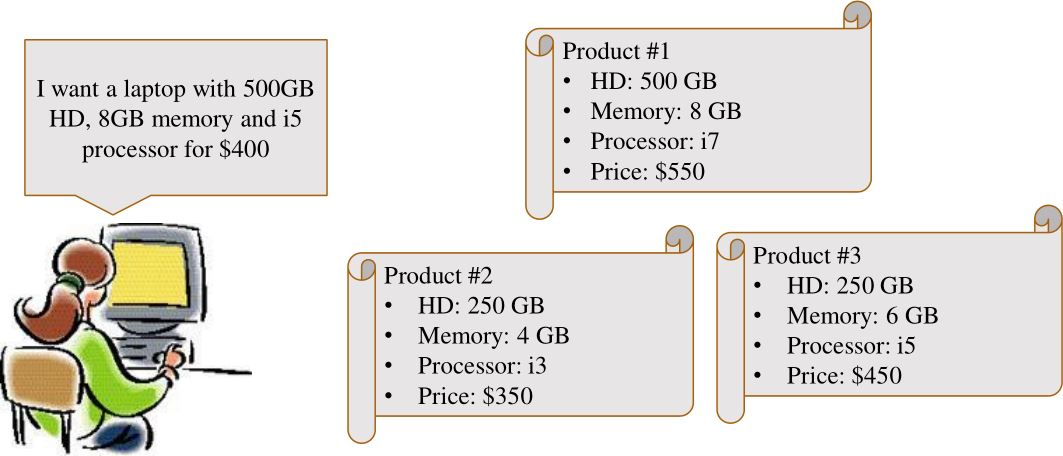
\includegraphics[height=2in]{imperfectmatchrecommendationsystem}
		\caption[Perfect matching recommendation may not exist]{Perfect matching recommendation may not exist.}
		\label{fig:imperfectmatchrecommendationsystem}
	\end{figure}

Types of recommendation systems
	\begin{bulletedlist}
		\item Popularity based recommendations
		\item Classification model based
		\item Content based recommendations
		\item Nearest neighbor collaborative filtering:
		\begin{bulletedlist}
			\item User based
			\item Item based
		\end{bulletedlist}
		\item Hybrid approaches
		\item Association rule mining
	\end{bulletedlist}

Popularity based Recommender System
	\begin{bulletedlist}
		\item Popularity based recommendation system works by recommending items viewed/pur\-chased by most people and rated high.
		\item Recommendations: Ranked list of items by their purchase count/viewed count.
		\item``Popular News''
		\begin{bulletedlist}
			\item Can use context
			\item Purchase history
			\item User and item features
			\item Scalable
		\end{bulletedlist}
		\item Not a personalized recommendation
	\end{bulletedlist}

	\section{Classification model}
	\begin{bulletedlist}
		\item Uses features of both products as well as users in order to predict whether a user will like a product or not.
		\item Limitation
		\begin{numberedlist}
			\item It is not easy to collect quality information about products and users.
			\item Even if we are able to collect good information, they may not be sufficient to make a good classifier.
			\item Scalability issue.
		\end{numberedlist}
	\end{bulletedlist}

	\begin{figure}[tbh]
		\centering
		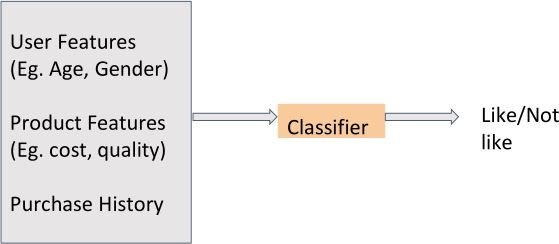
\includegraphics[height=2in]{recommendationsystemsclassificationmodel}
		\caption[Classification model]{Classification model.  The outcome can be 1 if the user likes it else 0 and it incorporates personalization.}
		\label{fig:recommendationsystemsclassificationmodel}
	\end{figure}

	\section{Content Based Recommendations}

	\begin{bulletedlist}
		\item Recommendations are based on information on the content of items rather than on other users' opinions.
		\item Main idea:
		\item If a user likes an item then he/she will also like a “similar” item
		\item Recommend items based on their similarity:
		\begin{bulletedlist}
			\item Recommend items to customer x similar to previous items rated highly by x.
		\end{bulletedlist}
		\item No need for data on other users.
		\begin{bulletedlist}
			\item No cold-start or sparsity problems.
		\end{bulletedlist}
		\item Able to recommend to users with unique tastes.
		\item Techniques that can be used: Cosine similarity.
	\end{bulletedlist}

	\section{Content Based Recommendation System}

	\begin{bulletedlist}
		\item Item Profiles:
		\begin{bulletedlist}
			\item set of features
			\item vector
		\end{bulletedlist}
		\begin{bulletedlist}
			\item Weighted average of rated item profiles
			\item Normalize rating using average rating of user.
		\end{bulletedlist}
		\item Advantages
		\begin{bulletedlist}
			\item Content-based recommender systems don't require a lot of user data.
			\item We just need item data and you're able to start giving recommendations to users.
			\item Recommendation engine does not depend on lots of user data, so it is possible to give recommendations to even your first customer as long as you have adequate data to build his user profile. Does not suffer from cold start.
			\item Less expensive to build and maintain.
		\end{bulletedlist}
		\item Challenges
		\begin{bulletedlist}
			\item Your item data needs to be well distributed.
			\item Availability of features which explain Items and user preferences.
			\item Recommendations will likely be direct substitutes, and not complements, of the item the user interacted with.  This is one of the key reasons why collaborative filtering provides better recommendations.
			\item Less dynamic.
		\end{bulletedlist}
	\end{bulletedlist}

	\begin{figure}
		\centering
		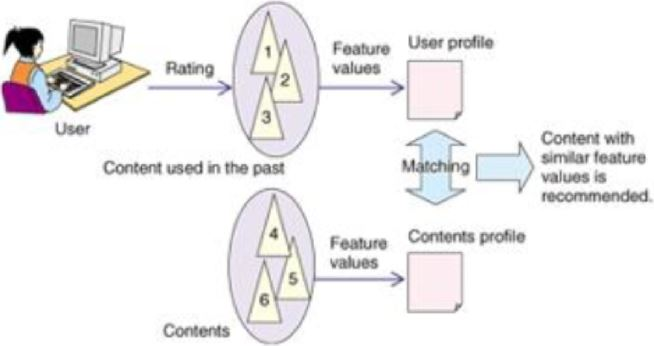
\includegraphics[width=2in]{contentbaserecommendationsystem}
		\caption[Content based recommendation system]{Content based recommendation system.}
		\label{fig:contentbaserecommendationsystem}
	\end{figure}

	\section{Cosine Similarity}
	\begin{bulletedlist}
		\item Cosine Similarity is the cosine of the angle between the 2 vectors A and B
		\item Closer the vectors, smaller will be the angle and hence larger their cosine value.
	\end{bulletedlist}

	\begin{equation}\label{eqn:cosinesimilarity}
		CosSim(x,y) = \frac{\sum_i x_i y_i}{\sqrt{\sum_i x_i^2}\sqrt{\sum_i y_i^2}} = \frac{\langle x,y\rangle}{\|x\|\|y\|}
	\end{equation}